\appendix

\chapter{Dokumentasi \emph{Screenshot} Presentasi Bersama \emph{Owner} Klinik \emph{Moist Care}}

\begin{figure}[H]
	\centering
	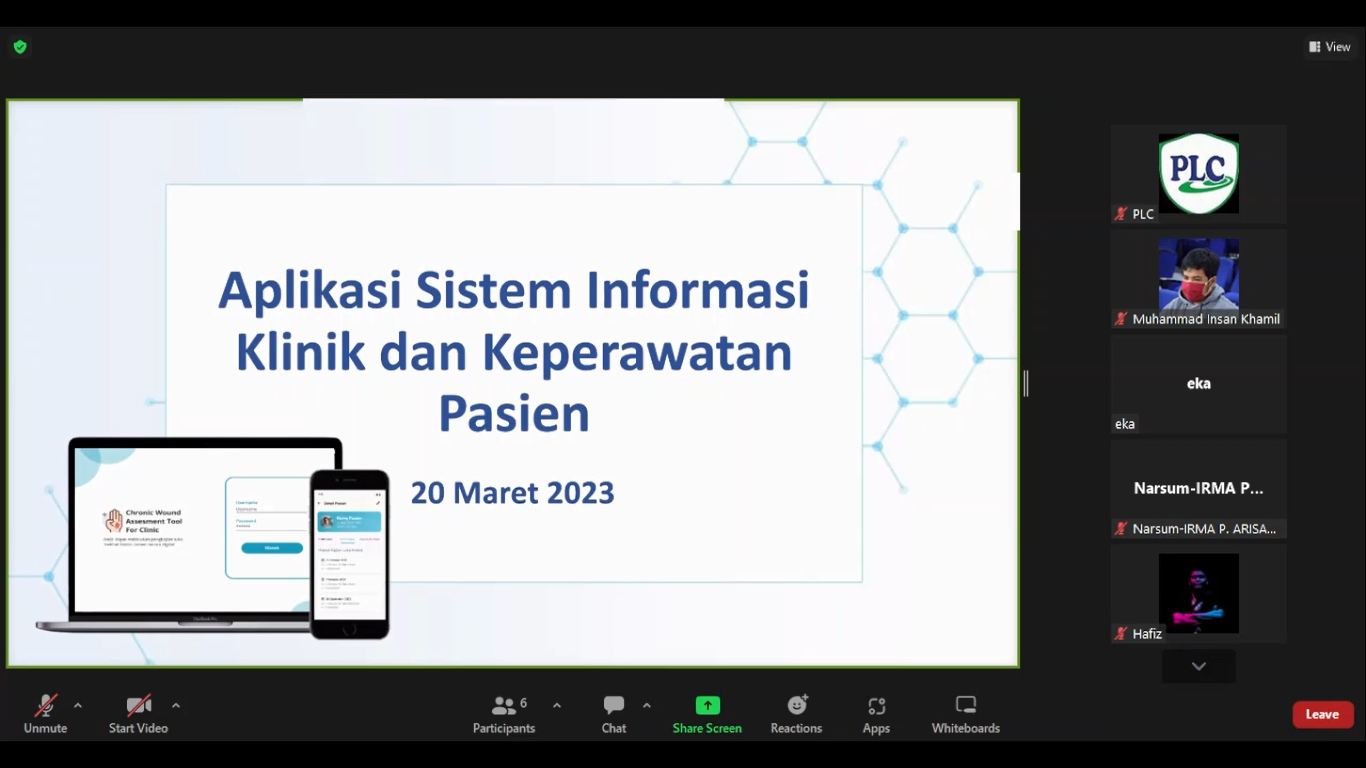
\includegraphics[width=12cm]{gambar/lampiranbuktipresentasi.png}
	\caption{Dokumentasi presentasi bersama Ibu Irma Puspita Arisanti 1} 
	\label{Gambar:usecaseadminjurnalpertama}
\end{figure}

\begin{figure}[H]
	\centering
	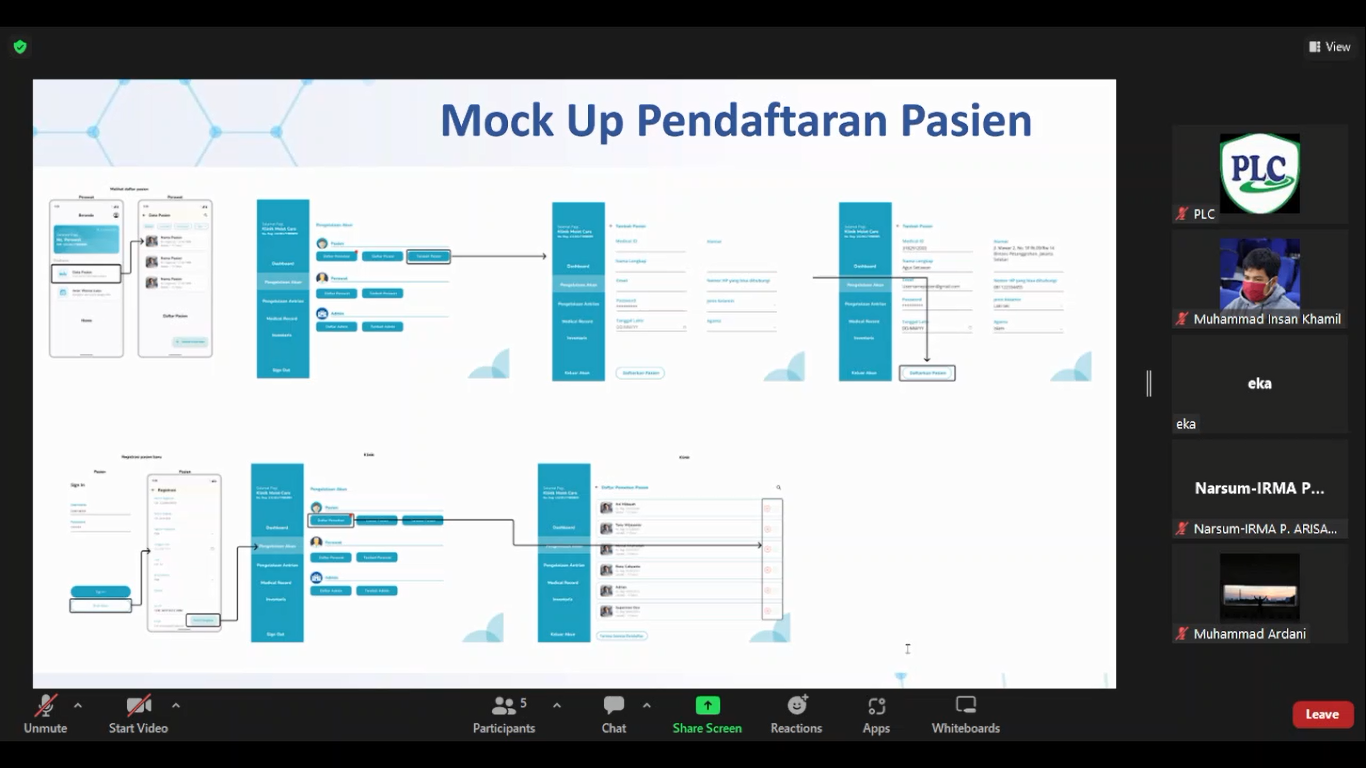
\includegraphics[width=12cm]{gambar/lampiranbuktipresentasi1.png}
	\caption{Dokumentasi presentasi bersama Ibu Irma Puspita Arisanti 2} 
	\label{Gambar:usecaseadminjurnalpertama}
\end{figure}

\chapter{Transkrip Paparan Presentasi Bersama Pemilik Klinik \emph{Moist Care} 1}

%Rekaman Suara dapat diakses pada:

\begin{table}[h!]
	\centering
\begin{center}
		
\begin{tabular}{ p{2.8cm} p{11cm}}
	
Narasumber & : Ibu Irma Puspita Arisanti\\

&\\

Narasumber & : Terkait penelitiannya kalau untuk saya bisa kasih masukan ini kan pak eka kan tadi gambarannya di PPT itu masih yang terlalu umum ya, saya gak lihat isinya, kalau mau saya lihat isinya begitu jadi nanti saya tahu ini ke sini, yang kemarin saya kasih gambaran kan kaya misalnya intinya ini buat siapa aplikasinya, buat pasien atau buat perawatnya atau buat instansi dimana perawat itu bekerja. Kalau misalnya untuk pasien berarti kan nanti kita informasinya seperti yang kemarin saya bilang itu, pasien itu paling enggak dapet informasi terkait dengan jadwal, cara dia bikin janji, kemudian melihat jadwal, melihat perkembangan lukanya, lalu kemudian lihat lukanya. Lihat perkembangan itu kan ini kemaren pakai versi insan ya, berarti kan ada skoring, nah skoring itu supaya melihat dia baik atau enggak kan ada grafik, kalau bisa tambahin ada grafiknya, itu yang di lihat pasien itu saja empat poin\\
	
\emph{Scrum Master} & : Kalau pengembangan sistem itu di bagi dua, pertama itu adalah daftar tertulis dari kebutuhan yang mau didevelop, kedua itu setelah dapat tertulis, biasanya kan ini tanda tangan, setelah butuh tanda tangan nanti ad kami ada dalam bentuk rancangan tatap muka. tapi kan kalau misalkan mau ada teks nanti kan gak kebayang kan, jadi nanti gini saja deh kita buat semua user interface, saya tampilkan semuanya\\

Narasumber & : Ya kan ini maksudnya apa ada tambahan atau ada yang mau dikurangin, nah kalau saya mau melihat yang di tambah dan apa yang di kurangi kalau dari PPT itu kemaren gak cukup, saya bingung itu loh, ya terserahlah mekanismenya bagaimana, yang terpenting tergambar alurnya, proses yang sudah terjadi dari awal sampai akhir, kalau itu kan satu slide sendiri, bicara tentang itu dan terlalu kecil-kecil dan saya tidak cukup memahami dari poin-poin itu. Terus kemudian bisa gak sih si perawatnya melihat rekapan kunjungan datanya itu misalnya muncul satu nama 

\end{tabular}

\end{center}
\end{table}
\break
\begin{table}[ht!]
	\centerfirst
\begin{center}
		
\begin{tabular}{ p{2.8cm} p{11cm}}
& kemudian dari satu nama itu ada muncul kontrol tanggal sekian tanggal sekian sampai sembuh, itu bisa apa enggak? Harusnya sih bisa, kebayang ya? Jadi kalau misalnya data pasien itu di klik pasien anu itu misalnya di klik itu rekapan kunjungannya dari awal sampai ke medical history perpasien. Jadi gak sekedar kita upload data, abis itu kita bingung ini ngeliat dari kunjungan pertama sampai terakhir itu gak bisa kita baca, ya kan itu history kan perawatan. Jadi satu pasien itu muncul ketika kita klik nama pasien muncul deh historynya mulai dari kunjungan satu sampai kunjungan sembuh, kalau perlu sampai ada pemeriksaan labnya, lampirannya di situ ada, termasuk foto lukanya juga ada di situ\\

\emph{Scrum Master} & : Kalau lab saya belum kebayang ya soalnya selama ini belum ada.\\

Narasumber & : Kalau begitu gak usah lah kalau belum mah, kalau bisa, berarti Cuma foto saja\\

\emph{Scrum Master} & : Yang penting kami butuh data sih\\

Narasumber & : Kalau data kita gak bisa kasih mas, karena kan itu kan ini bersifat privasi ya\\

\emph{Scrum Master} & : Maksudnya bukan data bu, melainkan proses alur klinik\\

Narasumber & : Data proses ya tadi yang saya sampaikan, data proses. Itu paling tambahan tambahannya kalau mau memasukkan lagi nanti bisa dilihat dari apa yang sudah ada yang perlu nanti bisa di tambahkan atau di kurangi\\
\end{tabular}

\end{center}
\end{table}

\chapter{Transkrip Paparan Presentasi Bersama Pemilik Klinik \emph{Moist Care} 2}

\begin{table}[h!]
	\centering
\begin{center}
		
\begin{tabular}{ p{2.8cm} p{11cm}}
	
Narasumber & : Ibu Irma Puspita Arisanti\\

&\\
			
Narasumber & : untuk penelitian saya oke-oke saja, nah ini untuk yang pra-penelitian kalau saya pikir prosedurnya sama kaya penelitian saja pak, kaya misalkan kaya alur penelitian kan membicarakan misalnya harga, validasi, prototipe, dua kali seminggu, dua pekan misalnya, itu kan masuk dalam model penelitian nanti kan, nanti mungkin yang ke kita penelitian itu surat penelitian, formal, kemudian proposal penelitiannya segala macam dilampirkan termasuk uji etic, karena kan kaitannya kita ngambil data pasien ya kan, nanti eticnya bagaimana, biasanya dari kampus kan, bapak konsultasi dulu ya karena kan terkait data-data pasien kan, begitu saja mungkin untuk yang penelitian prosedurnya, sampai ke alur kan, nanti kan di alur kan jelas tu step by step dari pihak peneliti, kemudian dari pihak kita apa. Paling itu sih ya pak sigit\\

\emph{Scrum master} & : jadi nanti kita minta izin ke bu irma untuk mengirim online ini nanti kita butuh validasi untuk pengembangan itu apakah cukup valuable di klinik atau enggak, mumpung kita masih awal development. Kalau misalkan sudah jalan itu nanti jadi sulit lagi\\

Narasumber & : jadi kaya kalau bahasanya modul ya, main modul, istilahnya modul kan?\\

\emph{Scrum master} & : saya kirim dokumen saja deh ke bu irma atau  nanti tolong dipelajari dulu lalu kalau butuh presentasi, nanti rekan-rekan paparkan lagi secara online gak papa kok\\

Ibu Irma & : ini untuk yang penelitian\\

\emph{Scrum master} & : penelitian mau kita belokin ke bisnis bu\\

Ibu Irma & : yang bahasan pertama ini yang penelitian yang di kirim ke saya kan?\\

\emph{Scrum master} & : tapi fiturenya yang sudah berbasis klinik, jadi klinik butuh apa itu harus di ceklist bu, minimal kerjanya ceklist saja deh\\
			
\end{tabular}
		
\end{center}
\end{table}

%Rekaman Suara dapat diakses pada: shorturl.at/ckmyO

\chapter{Surat Pernyataan Kesediaan Kerjasama Dari Mitra}

\begin{figure}[H]
	\centering
	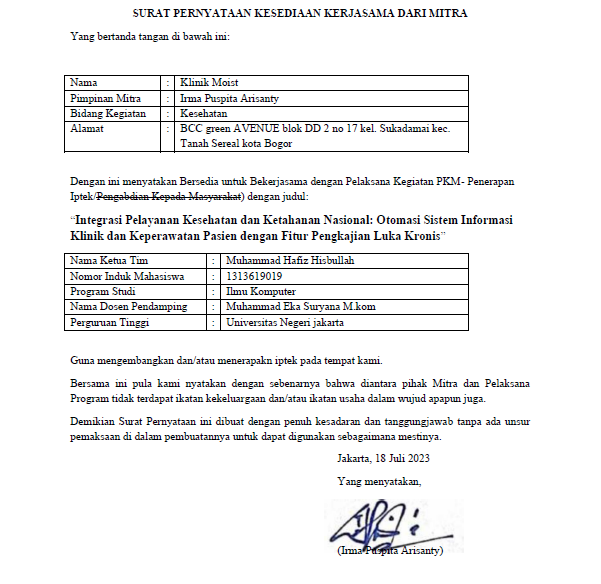
\includegraphics[width=16cm]{gambar/0024.png}
	\caption{Surat Pernyataan Kesediaan Kerjasama Dari Mitra}
	\label{Gambar:pengelolaanantrian2}
\end{figure}

\chapter{\emph{Code} Untuk \emph{View Login} Admin dan Perawat}

\begin{lstlisting}
	
	<!DOCTYPE html>
	<html lang="en">
	<head>
	<meta charset="utf-8">
	<meta http-equiv="X-UA-Compatible" content="IE=edge">
	<meta name="viewport" content="width=device-width,
	initial-scale=1, shrink-to-fit=no">
	<meta name="description" content="">
	<meta name="author" content="">
	<title>Sistem Informasi Keperawatan Luka -
	Login</title>
	<link
	href="https://fonts.googleapis.com/css?family=Nunito:2
	0,200i,300,300i,400,400i,600,600i,700,700i,800,800i,90
	,900i"
	rel="stylesheet">
	<!-- Custom styles for this template-->
	<link href="../static/css/sb-admin-2.min.css"
	rel="stylesheet">
	</head>
	<body>
	<div class="container">
	<!-- Outer Row -->
	<div class="row justify-content-center">
	<div class="col-xl-10 col-lg-12 col-md-9">
	<div class="border-0 my-7">
	<div class="card-body p-0">
	<!-- Nested Row within Card Body -->
	<div class="row">
	<div class="card col-lg-5 d-none d-lg-block border-0
	bg-login-image"></div>
	<div class="card col-lg-2 border-0"></div>
	<div class="card col-lg-5 border-1">
	<div class="p-5">
	<div class="text-center">
	<h1 class="h4 text-gray-900 mb-4">Sistem Informasi
	Keperawatan Luka</h1>
	</div>
	  
	  
	  
	<p>{{ message }}</p>  
	  
	  
	
	<form class="user" method="POST" action="/login">
	<div class="form-group">
	<input type="email" class="form-control
	form-control-user" name="email"
	id="username" placeholder="Enter Email Address" required>
	</div>
	<div class="form-group">
	<input type="password" class="form-control
	form-control-user" name="passw"
	id="passw" placeholder="Password" required>
	</div>
	<div class="form-group">
	<label class="text-gray-900" for="role">Login
	sebagai</label>
	<br>
	<input type="radio" name="role" id="admin"
	value="admin" required>
	<label for="html">Admin</label>&nbsp;
	<input type="radio" name="role" id="perawat"
	value="perawat" required>
	<label for="html">Perawat</label>
	</div>
	<button type="submit" class="btn btn-primary btn-user
	btn-block">
	Login
	</button>
	</form>
	</div>
	</div>
	</div>
	</div>
	</body>
	</html>
\end{lstlisting}

\chapter{\emph{Code} Untuk \emph{Web Service Login}  Admin dan Perawat}

\begin{lstlisting}
	@bp.route('/login', methods=['POST'])
	def login():
	try:
	data = { 
		"email" : request.form['email'], 
		"passw" : request.form['passw'],
		"role" : request.form['role']}
	a = db.get_user(data)
	if a == None:
	print("User tidak ditemukan")
	flash("User tidak ditemukan")
	return redirect(url_for('login'))
	else:
	session['user_info'] = {
		"email" : data["email"],
		"role" : data["role"]}
	print("Berhasil Login")
	flash("Berhasil Login")
	return redirect(url_for('home'))
	except Exception as ex:
	print("Gagal login")
	flash("Gagal login")
	return redirect(url_for('login'))
\end{lstlisting}

\chapter{\emph{Code} Untuk \emph{Dashboard} Klinik}

\begin{lstlisting}
	
	 Dashboard  
	
	<!-- Content Wrapper -->
	<div id="content-wrapper" class="d-flex flex-column
	my-0">
	<!-- Begin Page Content -->
	<div class="container">
	<!-- Outer Row -->
	<div class="row justify-content-center">
	<div class="card-body">
	<div class="text-left">
	<h1 class="h4 text-gray-900 my-3">Dashboard Klinik</h1>
	</div>
	  
	  
	  
	<p>{{ message }}</p>  
	  
	  
	 
	<!-- Nested Row within Card Body -->
	<div class="row">
	<div class="col-lg-12">
	<div class="p-5">
	<!-- Content Row -->
	<div class="row">
	<div class="col-xl-10 col-md-6 mb-4">
	<a href="#" class="d-none d-sm-inline-block btn btn-sm
	btn-primary shadow-sm"><i
	class="fas fa-sm text-white-50"></i> Kinerja
	Perawat</a>
	<a href="#" class="d-none d-sm-inline-block btn btn-sm
	btn-primary shadow-sm"><i
	class="fas fa-sm text-white-50"></i> Cost Perawatan
	Pasien</a>
	<a href="#" class="d-none d-sm-inline-block btn btn-sm
	btn-primary shadow-sm"><i
	class="fas fa-sm text-white-50"></i> Income Masuk</a>
	<a href="#" class="d-none d-sm-inline-block btn btn-sm
	btn-primary shadow-sm"><i
	class="fas fa-sm text-white-50"></i> Balance
	Keuangan</a>
	</div>
	</div>
	<div class="row">
	<!-- Area Chart -->
	<div class="col-xl-8 col-lg-7">
	<div class="card shadow mb-4">
	<!-- Card Header - Dropdown -->
	<div
	class="card-header py-3 d-flex flex-row
	align-items-center justify-content-between">
	<h6 class="m-0 font-weight-bold text-primary">Cost
	Perawatan Pasien</h6>
	<div class="dropdown no-arrow">
	<a class="dropdown-toggle" href="#" role="button"
	id="dropdownMenuLink"
	data-toggle="dropdown" aria-haspopup="true"
	aria-expanded="false">
	</a>
	</div>
	</div>
	<!-- Card Body -->
	<div class="card-body">
	<div class="chart-area">
	<canvas id="myAreaChart"></canvas>
	</div>
	</div>
	</div>
	</div>
	</div>
	</div>
	<!-- /.container-fluid -->
	</div>
	<!-- End of Main Content -->
	</div>
	</div>
	
\end{lstlisting}

\chapter{\emph{Code} Untuk \emph{Web Service Login} Pasien}

\begin{lstlisting}
	#login pasien
	@bp.route('/login_pasien', methods=['POST'])
	def login_pasien():
	try:
	data = { 
		"email" : request.form['email'], 
		"password" : request.form['passw'],
		"verif" : '1'
	}
	a = db.get_pasien_login(data)
	if a == None:
	print("Pasien tidak ditemukan")
	return Response(response = json.dumps({"message" :
		"failed"}), mimetype="application/json", status=400)
	else:
	print("Berhasil login")
	return Response(response = json.dumps({"message" :
		"success"}), mimetype="application/json", status=200)
	except Exception as ex:
	print (ex)
	return Response(response = json.dumps({"message" :
		"exe"}), mimetype="application/json", status=500)
\end{lstlisting}

\chapter{\emph{Code} Untuk \emph{View} Registrasi Pasien Dari Klinik}

\begin{lstlisting}
	
	
	 Tambah Pasien Baru  
	
	
	
	<!-- Content Wrapper -->
	<div id="content-wrapper" class="d-flex flex-column my-0">
	
	<!-- Begin Page Content -->
	<div class="container">
	
	<!-- Outer Row -->
	<div class="row justify-content-center">
	
	<div class="card-body">
	<div class="text-left">
	<h1 class="h4 text-gray-900 my-3">Tambah Pasien
	Baru</h1>
	</div>
	  
	  
	  
	<p>{{ message }}</p>  
	  
	  
	 
	<!-- Nested Row within Card Body -->
	<div class="row">
	<div class="col-lg-12">
	<div class="p-5">
	<form class="user" method="POST" action="/pasien">
	<div class="form-group row">
	<div class="col-sm-6">
	<label class="text-gray-900" for="email">Email*</label>
	<input type="email" class="form-control
	form-control-user" name="email"
	id="email aria-describedby="emailHelp"
	placeholder="Enter Email Address" required>
	</div>
	<div class="col-sm-6">
	<label class="text-gray-900"
	for="passw">Password*</label>
	<input type="password" class="form-control
	form-control-user" name="passw" minlength="8"
	maxlength="16"
	id="passw" placeholder="Enter Password" required>
	</div>
	</div>
	<div class="form-group row">
	<div class="col-sm-6">
	<label class="text-gray-900" for="nik">NIK*</label>
	<input type="number" class="form-control
	form-control-user" minlength="16" name="nik"
	id="nik" placeholder="Enter NIK" required>
	</div>
	<div class="col-sm-6">
	<label class="text-gray-900" for="nama">Nama*</label>
	<input type="text" class="form-control
	form-control-user" name="nama"
	id="nama" placeholder="Enter Name" required>
	</div>
	</div>
	<div class="form-group row">
	<div class="col-sm-6">
	<label class="text-gray-900" for="born_date">Tanggal
	Lahir*</label>
	<input type="date" class="form-control
	form-control-user" name="born_date"
	id="born_date" required>
	</div>
	<div class="col-sm-6">
	<label class="text-gray-900" for="usia">Usia*</label>
	<input type="number" class="form-control
	form-control-user" name="usia"
	id="usia" placeholder="Enter Age" required>
	</div>
	</div>
	<div class="form-group row">
	<div class="col-sm-6">
	<label class="text-gray-900" for="kelamin">Jenis
	Kelamin*</label>
	<br>
	<input type="radio" name="kelamin" id="laki-laki"
	value="laki-laki" required>
	<label for="html">Laki-laki</label><br>
	<input type="radio" name="kelamin" id="perempuan"
	value="perempuan" required>
	<label for="html">Perempuan</label><br>
	</div>
	<div class="col-sm-6">
	<label class="text-gray-900"
	for="kelamin">Agama*</label>
	<br>
	<input type="radio" name="agama" id="islam"
	value="islam" required>
	<label for="html">Islam</label><br>
	<input type="radio" name="agama" id="kristen"
	value="kristen" required>
	<label for="html">Kristen</label><br>
	<input type="radio" name="agama" id="hindu"
	value="hindu" required>
	<label for="html">Hindu</label><br>
	<input type="radio" name="agama" id="buddha"
	value="buddha" required>
	<label for="html">Buddha</label><br>
	<input type="radio" name="agama" id="konghucu"
	value="konghucu" required>
	<label for="html">Konghucu</label><br>
	</div>
	</div>
	<div class="form-group row">
	<div class="col-sm-6">
	<label class="text-gray-900"
	for="alamat">Alamat*</label>
	<input type="text" class="form-control
	form-control-user" name="alamat"
	id="alamat" placeholder="Enter Address" required>
	</div>
	<div class="col-sm-6">
	<label class="text-gray-900" for="no_hp">Nomor
	Handphone*</label>
	<input type="number" class="form-control
	form-control-user" name="no_hp"
	id="no_hp" placeholder="Enter handphone number" required>
	</div>
	</div>
	<div class="form-group row">
	<div class="col-sm-6">
	<label class="text-gray-900" for="no_bpjs">Nomor
	BPJS</label>
	<input type="number" class="form-control
	form-control-user" name="no_bpjs"
	id="no_bpjs" placeholder="Enter BPJS Number">
	</div>
	</div>
	<div class=" row">
	<div class="col-sm-3">
	<a class="btn btn-primary btn-user btn-block"
	href="{{url_for('manage_accounts')}}">
	Kembali</button>
	</a>
	</div>
	<div class="col-sm-3"></div>
	<div class="col-sm-3"></div>
	<div class="col-sm-3">
	<button type="submit" class="btn btn-primary btn-user
	btn-block">
	Submit</button>
	</div>
	</div>
	</form>
	</div>
	</div>
	</div>
	</div>
	</div>
	</div>
	<!-- /.container-fluid -->
	</div>
	<!-- End of Main Content -->
	
\end{lstlisting}

\chapter{\emph{Code} Untuk \emph{Web Service} Registrasi Pasien Dari Klinik}

\begin{lstlisting}
	@bp.route('/pasien', methods =['POST'])
	def addpasien():
	try:       
	data = {"email": request.form['email'],
		"password": request.form['passw'],
		"nik": request.form['nik'],
		"nama":request.form['nama'],
		"kelamin": request.form['kelamin'],
		"agama":request.form['agama'],
		"born_date":request.form['born_date'],
		"usia":request.form['usia'],
		"alamat": request.form['alamat'],
		"no_hp": request.form['no_hp'],
		"created_at" : time.strftime("%d/%m/%Y %H:%M:%S"),
		"updated_at" : time.strftime("%d/%m/%Y %H:%M:%S"),
		"list_image_id": [],
		"verif": '1'}
	cek = get_pasien(data)
	if cek == None:
	row = insert_pasien(data)
	print("Berhasil input pasien baru")
	flash("Berhasil input pasien baru")
	return redirect(url_for('add_new_patient'))
	else:
	print("Gagal input pasien baru")
	flash("Gagal input pasien baru")
	return redirect(url_for('add_new_patient'))
	except Exception as ex:
	print("Gagal input pasien baru")
	flash("Gagal input pasien baru")
	return redirect(url_for('add_new_patient'))
\end{lstlisting}

\chapter{\emph{Code} Untuk \emph{View List} Permohonan Akun Pasien}

\begin{lstlisting}
	
	 Daftar Permohonan Pasien Baru
	 
	
	<!-- Content Wrapper -->
	<div id="content-wrapper" class="d-flex flex-column
	my-0">
	<!-- Begin Page Content -->
	<div class="container-fluid">
	<!-- Outer Row -->
	<div class="row justify-content-center">
	<div class="card-body">
	<div class="text-left">
	<h1 class="h4 text-gray-900 my-3">Daftar Permohonan
	Pasien Baru</h1>
	</div>
	  
	  
	  
	<p>{{ message }}</p>  
	  
	  
	
	<!-- DataTales Example -->
	<div class="card mb-4">
	<div class="card-body">
	<div class="table-responsive">
	<table class="table table-bordered" id="dataTable"
	width="100%" cellspacing="0">
	<thead>
	<tr>
	<th>NIK</th>
	<th>Nama</th>
	<th>Jenis Kelamin</th>
	<th>Usia</th>
	<th>Action</th>
	</tr>
	</thead>
	<tbody>
	
	<tr>
	<td>{{ item.nik }}</td>
	<td>{{ item.nama }}</td>
	<td>{{ item.kelamin }}</td>
	<td>{{ item.usia }}</td>
	<td><a class="btn btn-primary btn-user btn-block"
	href="{{url_for('profil_pemohon_pasien_baru', _id =
			item._id )}}">
	lihat</a>
	</td>
	</tr>
	
	</tbody>
	</table>
	</div>
	<div class=" row">
	<div class="col-sm-3">
	<a class="btn btn-primary btn-user btn-block"
	href="{{url_for('manage_accounts')}}">
	Kembali</button>
	</a>
	</div>
	<div class="col-sm-3"></div>
	<div class="col-sm-3"></div>
	<div class="col-sm-3"></div>
	</div>
	</div>
	</div>
	</div>
	</div>
	</div>
	<!-- /.container-fluid -->
	</div>
	<!-- End of Main Content -->
	
\end{lstlisting}

\chapter{\emph{Code} Untuk \emph{Web Service} \emph{List} Permohonan Akun Pasien}

\begin{lstlisting}
	#akses semua pasien yang belum terverifikasi klinik
	@bp.route('/pasien_unverify', methods =['GET'])
	def get_pasiens_unverify():
	a = db.get_pasiens_unverify()
	a_serializable = [{'_id': str(patient['_id']),
		'email':patient['email'], 'nama':patient['nama'],
		'born_date':patient['born_date'],
		'usia':patient['usia'], 'kelamin':patient['kelamin'],
		'agama':patient['agama'], 'alamat':patient['alamat'],
		'no_hp':patient['no_hp'], 'nik':patient['nik']} for
	patient in a]
	print("pass")
	return Response(response =
	json.dumps(list(a_serializable)),
	mimetype="application/json", status=200)
\end{lstlisting}

\chapter{\emph{Code} Untuk \emph{Web Wervice List} Verifikasi/Terima pasien}

\begin{lstlisting}
	#akses merubah pasien belum terverifikasi menjadi pasien
	terverifikasi
	@bp.route('/accept_verif_pasien/<_id>', methods =['GET'])
	def accept_unverify_patient(_id):
	a = db.verify_pasien(_id)
	print("pass")
	flash("Berhasil verifikasi pasien")
	return redirect(url_for('list_request_new_patient'))
\end{lstlisting}

\chapter{\emph{Code} Untuk \emph{Web Service List} Tolak Verifikasi Pasien}

\begin{lstlisting}
	#akses merubah pasien belum terverifikasi menjadi 
	pasien terblokir
	@bp.route('/block_verif_pasien/<_id>', methods=
	['GET'])
	def block_unverify_patient(_id):
	a = db.block_pasien(_id)
	print("pass")
	flash("Berhasil blokir pasien")
	return redirect(url_for('list_request_new_patient'))
\end{lstlisting}

\chapter{\emph{Code} Untuk \emph{View List} Pasien Terdaftar Klinik}

\begin{lstlisting}
	
	 Daftar Pasien 
	
	<div id="content-wrapper" class="d-flex flex-column 
	my-0">
	<div class="container-fluid">
	<div class="row justify-content-center">
	<div class="card-body">
	<div class="text-left">
	<h1 class="h4 text-gray-900 my-3">Daftar Pasien</h1>
	</div>
	<div class="card-body">
	<div class="table-responsive">
	<table class="table table-bordered" id="dataTable"
	width="100%" cellspacing="0">
	<thead>
	<tr>
	<th>NIK</th>
	<th>Nama</th>
	<th>Jenis Kelamin</th>
	<th>Usia</th>
	<th>action</th>
	</tr>
	</thead>
	<tbody>
	
	<tr>
	<td>{{ item.nik }}</td>
	<td>{{ item.nama }}</td>
	<td>{{ item.kelamin }}</td>
	<td>{{ item.usia }}</td>
	<td><a class="btn btn-primary btn-user btn-block"
	href="{{url_for('profil_pasien', _id = item._id
			)}}">lihat</a></td>
	</tr>
	
	</tbody>
	</table>
	</div>
	<div class=" row">
	<div class="col-sm-3">
	<a class="btn btn-primary btn-user btn-block"
	href="{{url_for('manage_accounts')}}">
	Kembali</button>
	</a>
	</div>
	<div class="col-sm-3"></div>
	<div class="col-sm-3"></div>
	<div class="col-sm-3"></div>
	</div>
	
\end{lstlisting}

\chapter{\emph{Code} Untuk \emph{Web Service List} Pasien Terdaftar Klinik}

\begin{lstlisting}
	#akses semua pasien yang telah terverifikasi klinik
	@bp.route('/pasien', methods =['GET'])
	def get_pasiens():
	a = db.get_pasiens()
	a_serializable = [{'_id': str(patient['_id']),
		'email':patient['email'], 'nama':patient['nama'],
		'born_date':patient['born_date'],
		'usia':patient['usia'], 'kelamin':patient['kelamin'],
		'agama':patient['agama'], 'alamat':patient['alamat'],
		'no_hp':patient['no_hp'], 'nik':patient['nik']} for
	patient in a]
	return Response(response =
	json.dumps(list(a_serializable)),
	mimetype="application/json", status=200)
\end{lstlisting}

\chapter{\emph{Code} Untuk \emph{View} Detail Hasil Pemeriksaan Kesehatan}

\begin{lstlisting}
	
	 Hasil Pemeriksaan 
	Kesehatan  
	
	<div id="content-wrapper" class="d-flex flex-
	column my-0">
	<div class="container">
	<div class="row justify-content-center">
	<div class="card-body">
	<div class="text-left">
	<h1 class="h4 text-gray-900 my-3">Hasil 
	Pemeriksaan Kesehatan</h1>
	</div>
	<div class="row">
	<div class="col-lg-12">
	<div class="p-5">
	
	<div class=" row">
	<div class="col-sm-6">
	<label class="text-gray-900" for="tanggal">
	Tanggal Pemeriksaan</label>
	<br>
	<label for="email">{{ item.tanggal }}</label>
	</div>
	</div>
	<br>
	<div class=" row">
	<div class="col-sm-6">
	<label class="text-gray-900" for="tekanan_
	darah">Tekanan Darah</label>
	<br>
	<label for="born_date">{{ item.tekanan_
			darah }}</label>
	</div>
	<div class="col-sm-6">
	<label class="text-gray-900" for="nadi">
	Nadi</label>
	<br>
	<label for="alamat">{{ item.nadi }}</label>
	</div>
	</div>
	<div class=" row">
	<div class="col-sm-6">
	<label class="text-gray-900" for="suhu">Suhu 
	Tubuh</label>
	<br>
	<label for="born_date">{{ item.suhu }}</label>
	</div>
	<div class="col-sm-6">
	<label class="text-gray-900" for="gula_darah
	_sewaktu">Gula Darah Sewaktu</label>
	<br>
	<label for="alamat">{{ item.gula_darah_
			sewaktu }}</label>
	</div>
	</div>
	<div class=" row">
	<div class="col-sm-6">
	<label class="text-gray-900" for="ABPI">
	ABPI</label>
	<br>
	<label for="born_date">{{ item.
			ABPI }}</label>
	</div>
	</div>
	<div class=" row">
	<div class="col-sm-3">
	<a type="submit" class="btn btn-primary 
	btn-user btn-block" href="{{url_for('list
			_medical_check_data', nik=item.nik )}}">
	Back</a>
	</div>
	<div class="col-sm-3"></div>
	<div class="col-sm-3"></div>
	<div class="col-sm-3"></div>
	</div>
	
	</div>
	
\end{lstlisting}

\chapter{\emph{Code} Untuk \emph{Web Service} Tambah Hasil Pemeriksaan Kesehatan}

\begin{lstlisting}
	@bp.route('/add_data_pemeriksaan_kesehatan', 
	methods =['POST'])
	def post_data_pk():
	try:       
	a = list(get_data_pemeriksaan_kesehatan())
	data = {"_id": 100000000 + len(a) + 1,
		"tanggal": request.form['tanggal'],
		"username": request.form['username'],
		"nik": request.form['nik'],
		"tekanan_darah": request.form['tekan
		an_darah'],
		"nadi": request.form['nadi'],
		"suhu": request.form['suhu'],
		"gula_darah_sewaktu":request.form['
		gula_darah_sewaktu'],
		"ABPI" : request.form['ABPI']}
	insert_data_pemeriksaan_kesehatan(data) 
	print("Berhasil input data pemeriksaan kesehatan")       
	return Response(response = json.dumps(data), status=200)
	except Exception as ex:
	print("Gagal input data pemeriksaan kesehatan")  
	return Response(response = json.dumps({"message" : "error
		encountered"}), mimetype="application/json", status=500)
\end{lstlisting}

\chapter{\emph{Code} Untuk \emph{Web Service} Untuk Mendapatkan Detail Data Hasil Pemeriksaan Kesehatan Pasien Berdasar Tanggal Pemeriksaan}

\begin{lstlisting}
	@bp.route('/detail_data_pk_pasien/<_id>',
	methods =['GET'])
	def detail_data_pk(_id):
	a = get_detail_data_pemeriksaan_kesehatan
	_one_patient(_id)
	print(a)
	a_serializable = [a]
	return Response(response = json.dumps(list
	(a_serializable)), mimetype="application/json", 
	status=200)
\end{lstlisting}

\chapter{\emph{Code} Untuk \emph{View List} Inventaris}

\begin{lstlisting}
	
	 Inventaris 
	
	
	<div id="content-wrapper" class="d-flex flex-column 
	my-0">
	<h1 class="h4 text-gray-900 my-3">Inventaris</h1>
	</div>
	  
	  
	  
	<p>{{ message }}</p>  
	  
	  
	
	<div class="card mb-4">
	<div class="card-body">
	<div class="table-responsive">
	<table class="table table-bordered" id="dataTable"
	width="100%" cellspacing="0">
	<thead>
	<tr>
	<th>ID Inventaris</th>
	<th>Nama Inventaris</th>
	<th>Tipe Inventaris</th>
	<th>Harga</th>
	<th>Action</th>
	</tr>
	</thead>
	<tbody>
	
	<tr>
	<td>{{ item._id }}</td>
	<td>{{ item.nama_inventaris }}</td>
	<td>{{ item.tipe_inventaris }}</td>
	<td>{{ item.harga }}</td>
	<td><a class="btn btn-primary btn-user btn-block"
	href="{{url_for('detail_inventaris',
			_id = item._id )}}">lihat</a></td>
	</tr>
	
	</tbody>
	</table>
	</div>
	<div class=" row">
	<div class="col-sm-3">
	<a type="submit" class="btn btn-primary btn-user 
	btn-block" href="{{url_for('inventaris')}}">
	Tambah Inventaris</a>
	
\end{lstlisting}

\chapter{\emph{Code} Untuk \emph{View} Tambah Inventaris}

\begin{lstlisting}
	
	 Tambah Inventaris 
	 
	
	<div id="content-wrapper" class="d-flex flex-column 
	my-0">
	<h1 class="h4 text-gray-900 my-3">Tambah Inventaris 
	Baru</h1>
	</div>
	  
	  
	  
	<p>{{ message }}</p>  
	  
	  
	 
	<div class="row">
	<form class="user" method="POST" action="
	/inventaris">
	<div class="form-group row">
	<div class="col-sm-6">
	<label class="text-gray-900" for="nama_inventaris">
	Nama Inventaris*</label>
	<input type="text" class="form-control 
	form-control-user" name="nama_inventaris" 
	id="nama_inventaris" required>
	</div>
	<div class="col-sm-6">
	<label class="text-gray-900" for="keterangan">Keterangan*</label>
	<input type="text" class="form-control form-control-user"
	name="keterangan" id="keterangan" required>
	</div>
	</div>
	<div class="form-group row">
	<div class="col-sm-6">
	<label class="text-gray-900" for="harga">
	Harga*</label>
	<input type="number" class="form-control form-
	control-user" name="harga" id="harga" required>
	</div>
	<div class="col-sm-6">
	<label class="text-gray-900" for="harga">
	Jumlah*</label>
	<input type="number" class="form-control form-
	control-user"name="jumlah" id="jumlah" required>
	</div>
	</div>
	<div class="form-group row">
	<div class="col-sm-6">
	<label class="text-gray-900" for="tipe_inventaris">
	Tipe Inventaris*</label>
	<br>
	<input type="radio" name="tipe_inventaris" 
	id="obat" value="obat" required>
	<label for="html">Obat</label><br>
	<input type="radio" name="tipe_inventaris" 
	id="balutan" value="balutan" required>
	<label for="html">Balutan</label><br>
	</div>
	</div>
	<div class=" row">
	<div class="col-sm-3">
	<a class="btn btn-primary btn-user btn-block"
	href="{{url_for('list_inventaris')}}">
	Kembali</button>
	</a>
	</div>
	<div class="col-sm-3"></div>
	<div class="col-sm-3"></div>
	<div class="col-sm-3">
	<button type="submit" class="btn btn-primary
	btn-user btn-block">
	Submit</button>
	</div>
	</div>
	</form>
	</div>
	</div>
	
\end{lstlisting}

\chapter{\emph{Code} Untuk \emph{Web Service} Tambah Inventaris}

\begin{lstlisting}
	@bp.route('/inventaris', methods =['POST'])
	def addinventory():
	try:       
	data = {"nama_inventaris": request.form['nama_inventaris'],
		"tipe_inventaris": request.form['tipe_inventaris'],
		"harga": request.form['harga'],
		"keterangan":request.form['keterangan'],
		"jumlah" : request.form['jumlah']}
	cek = get_inventaris(data)
	if cek == None:
	row = insert_inventaris(data)
	print("berhasil input inventaris")
	flash("berhasil input inventaris")
	return redirect(url_for('inventaris'))
	else:
	#jika sudah ada data yang sama maka tidak 
	bisa daftar lagi
	print("gagal input inventaris")
	flash("gagal input inventaris")
	return redirect(url_for('inventaris'))
	except Exception as ex:
	print(ex)
	flash("gagal input inventaris")
	return redirect(url_for('inventaris'))
\end{lstlisting}

\chapter{\emph{Code} Untuk \emph{View List} Layanan}

\begin{lstlisting}
	
	 Layanan 
	 
	
	<div id="content-wrapper" class="d-flex flex-column my-0">
	<div class="container-fluid">
	<div class="row justify-content-center">
	<div class="card-body">
	<div class="text-left">
	<h1 class="h4 text-gray-900 my-3">Inventaris</h1>
	</div>
	  
	  
	  
	<p>{{ message }}</p>  
	  
	  
	
	<div class="card mb-4">
	<div class="card-body">
	<div class="table-responsive">
	<table class="table table-bordered" id="dataTable"
	width="100%" cellspacing="0">
	<thead>
	<tr>
	<th>ID Layanan</th>
	<th>Nama Layanan</th>
	<th>Harga</th>
	<th>Action</th>
	</tr>
	</thead>
	<tbody>
	
	<tr>
	<td>{{ item._id }}</td>
	<td>{{ item.nama_layanan }}</td>
	<td>{{ item.harga }}</td>
	<td><a class="btn btn-primary btn-user btn-block"
	href="{{url_for('detail_layanan', _id = item._id
			)}}">lihat</a></td>
	</tr>
	
	</tbody>
	</table>
	</div>
	<div class=" row">
	<div class="col-sm-3"></div>
	<div class="col-sm-3"></div>
	<div class="col-sm-3"></div>
	<div class="col-sm-3">
	<a type="submit" class="btn btn-primary btn-user btn-block"
	href="{{url_for('layanan')}}">
	Tambah Layanan</a>
	</div>
	</div>
	</div>
	</div>
	</div>
	</div>
	</div>
	</div>
	
\end{lstlisting}

\chapter{\emph{Code} Untuk \emph{View} Tambah Layanan}

\begin{lstlisting}
	
	 Tambah Layanan 
	 
	
	<div id="content-wrapper" class="d-flex flex-column 
	my-0">
	<div class="container">
	<div class="row justify-content-center">
	<div class="card-body">
	<div class="text-left">
	<h1 class="h4 text-gray-900 my-3">Tambah Layanan 
	Baru</h1>
	</div>
	  
	  
	  
	<p>{{ message }}</p>  
	  
	  
	
	<div class="row">
	<div class="col-lg-12">
	<div class="p-5">
	<form class="user" method="POST" action="/layanan">
	<div class="form-group row">
	<div class="col-sm-6">
	<label class="text-gray-900" for="nama_layanan">
	Nama Layanan*</label>
	<input type="text" class="form-control 
	form-control-user" name="nama_layanan"
	id="nama_layanan" required>
	</div>
	<div class="col-sm-6">
	<label class="text-gray-900"
	for="keterangan">Keterangan*</label>
	<input type="text" class="form-control 
	form-control-user" name="keterangan" id="keterangan" 
	required>
	</div>
	</div>
	<div class="form-group row">
	<div class="col-sm-6">
	<label class="text-gray-900" for="harga">
	Harga*</label>
	<input type="number" class="form-control 
	form-control-user" name="harga" id="harga" 
	required>
	</div>
	</div>
	<div class=" row">
	<div class="col-sm-3">
	<a class="btn btn-primary btn-user btn-
	block" href="{{url_for('list_layanan')}}">
	Kembali</button>
	</a>
	</div>
	<div class="col-sm-3"></div>
	<div class="col-sm-3"></div>
	<div class="col-sm-3">
	<button type="submit" class="btn btn-primary 
	btn-user btn-block">
	Submit</button>
	</div>
	</div>
	</form>
	</div>
	</div>
	</div>
	</div>
	</div>
	</div>
	</div>
	
\end{lstlisting}

\chapter{\emph{Code} Untuk \emph{Web Service} Tambah Layanan}

\begin{lstlisting}
	@bp.route('/layanan', methods =['POST'])
	def addservice():
	try:       
	data = {
		"nama_layanan": request.form['nama_layanan'],
		"keterangan": request.form['keterangan'],
		"harga":request.form['harga'],
	}
	cek = get_layanan(data)
	if cek == None:
	row = insert_layanan(data)
	print("Berhasil input layanan")
	flash("Berhasil input layanan")
	return redirect(url_for('layanan'))
	else:
	print("Gagal input layanan")
	flash("Gagal input layanan")
	return redirect(url_for('layanan'))
	except Exception as ex:
	print("Gagal input layanan")
	flash("Gagal input layanan")
	return redirect(url_for('layanan'))
\end{lstlisting}




\begin{comment}
	
\end{comment}

